\documentclass[12pt, letterpaper, titlepage]{report}
% \special{papersize=8.5in,11in}

% Import setup file with includes
\input{setup.tex}

%%%%%%%%%%%%%%%%%%%%%%%%%%%%%%%%%%%
% ---- Paper Specific Setup ----- %
%%%%%%%%%%%%%%%%%%%%%%%%%%%%%%%%%%%
\thispagestyle{plain}   % Makes title page have numbers
\pagestyle{plain}       % Makes other pages have numbers

\bibliography{ref}      % Add bibliography

\title{Development of a Customizable Bio-Mechanical Actuated Knee Orthosis for Exoskeletons Thesis}
% {\footnotesize to be used with Microsoft VSCode and Latex}

\author{\textbf{Alex C. Tacescu}}

% \affil{
% {Masters Thesis in Robotics Engineering} \\
% {Robotics Engineering Department} \\
% {Worcester Polytechnic Institute}
% }

\date{May 2021}

\makeatletter

\begin{document}

    % Make Title Page
    % \maketitle
    \begin{titlepage}
    \includegraphics[width=0.35\textwidth]{Figures/WPILogo.png} 
    \hspace{0.3\textwidth}
    \includegraphics[width=0.23\textwidth]{Figures/WPIAIMLogo.png}
    \begin{center}
        \setstretch{1.7}
        % Create Title 
        \rule{\linewidth}{1pt}
        \\[0.2cm]
        {\huge \textbf{\@title}}
        \\[0.1cm]
        \rule{\linewidth}{1pt}

        % Author
        \textsc{\LARGE \textbf{\@author}} \\
        \textsc{Submitted to the Faculty of}\\
        \textsc{\large \textbf{Worcester Polytechnic Institute}} \\
        \textsc{In partial fulfillment of the requirements for} \\
        \textsc{\large Degree of Masters in Science in Robotics Engineering}
    \end{center}
    \setstretch{1}
    Approved By:

    \vspace{1cm}
    \noindent\rule{0.6\linewidth}{0.4pt} \\
    \hspace{1cm} Thesis Advisor: Prof. Gregory Fischer

    \vspace{1cm}
    \noindent\rule{0.6\linewidth}{0.4pt} \\
    Committee Member: Dr. Christopher Nycz

    \vspace{1cm}
    \noindent\rule{0.6\linewidth}{0.4pt} \\
    \hspace{1cm} Committee Member: Prof. Karen Troy

    \vfill
    % Bottom of the page
    \begin{center}
        \large \@date
    \end{center}
             
 \end{titlepage}
    
    \doublespacing
    
    % \begin{abstract}
    %%%%%%%%%%%%%%%%%%%%%%%%%%%%
    % ---- Short Abstract ---- %
    %%%%%%%%%%%%%%%%%%%%%%%%%%%%

    % Current research demonstrates that the shank (lower leg) linearly extends as the knee flexes, in a roughly quartic trajectory. However, most actuated orthoses do not consider this tibiofemoral relationship. This thesis presents a customizable biomechanical orthotic knee joint for medical rehabilitation which can follow this relationship. The design is easily manufacturable with common machining tools and FDM 3D printing techniques. Most importantly, it is customizable to each patient with the simple replacement of one component. Finally, this thesis will present a software workflow and tools to identify this tibiofemoral relationship in patients using motion capture technologies. 

    %%%%%%%%%%%%%%%%%%%%%%%%%%%
    % ---- Long Abstract ---- %
    %%%%%%%%%%%%%%%%%%%%%%%%%%%

    Paraplegia - the loss of feeling and/or movement in one's lower limbs - affects hundred of thousands of people in the United States, and can be caused by spinal cord injury or diseases such as multiple sclerosis, stroke, and cancer. Paralysis patients can help alleviate side effects through physical therapy and rehabilitation. Gait training with exoskeletons may be particularly effective, with some clinical research reporting even fully paralyzed individuals reducing their side effects. However, orthoses used with these patients must be carefully designed to ensure safety and comfort and avoid rubbing between the orthosis and the patient's skin, as dermatological issues can often pose risks to these individuals due to the reduced sensation and blood flow to affected limbs.
    
    Current lower limb rehabilitation exoskeletons for gait training use pin joints for the 6 powered limbs (ankle, knee, and hip joints). However current research demonstrates that the shank (lower leg) linearly extends as the knee joint flexes. Tis tibiofemoral relationship is not usually considered by developers of lower limb orthoses.

    This thesis presents a customizable biomechanical knee orthosis for medical rehabilitation which follow a patient's specific knee trajectory. The design can be manufactured with common machining tools and FDM 3D printing techniques. It can also be customized to each patient with the replacement of a single component. The testing and analysis demonstrates that the proposed orthosis can match and exceed the requirements presented, and successfully matches a defined tibiofemoral relationship.

    Additionally, this thesis introduces a software workflow with motion capture systems to identify the knee joint parameters in a patient for customization of the proposed orthosis. The software developed was tested with pilot data to verify processes and improve the workflow presented. Finally, a clinical human trial is outlined to verify the effectiveness of the proposed orthosis, test the effectiveness of the software workflow, and identify the relationship between the knee joint and the surrounding skin using a mixture of motion capture data and magnetic resonance imaging.

\end{abstract}



    % % Affiliations

    % % Make Table of Contents
    \tableofcontents
    \listoffigures
    \listoftables

    \chapter{Introduction}
Paraplegia is a medical term used to define where a patient loses feeling and/or movement in their lower two limbs. In comparison, quadriplegia (also sometimes known as tetraplegia) is the loss of control in all four limbs. Sudden walking disabilities, such as lower limb paralysis, change a person's mobility, and often have quite a significant effect on a person's lifestyle and health. Not all feeling/movement needs to be lost in order for someone to be considered paraplegic \cite{IncompleteTraumaticQuadrilegia}. Only 30\% of all paraplegic and quadriplegic patients are considered complete lesions, where there is no sensation and no mobility in the lower limbs \cite{RehabParaplegia}. Paraplegia can introduce a significant challenge to maintain healthy bone and muscle mass, as the patient usually will have a much harder time exercising. However, research has shown that controlled rehabilitation can actually help reconnect a patient's injured neurons, reducing the effects of the injury and regaining mobility and/or feeling in their lower limbs \cite{GaitTrainingClinical}. As such, a large part of a paralysis victim's life is devoted to rehabilitation and physical therapy.

Exercises for rehabilitation come in many forms, from stretching to strength training, to hydrotherapy. Gait training has specifically been shown to improve the quality of life of a lower-limb paralysis patient, but this exercise is very hard to do, especially with severe cases of paraplegia. Robotics and exoskeletons have been proposed and tested to help with this cause. A mechanical system with intelligent software control can be used to assist and hold a person's weight as they perform exercises as called for by their doctor. Such systems can decrease bone and muscle atrophy and help fight the side effects of paraplegia. Robotics and image processing have a very large opportunity to improve the rehabilitation process in paraplegic patients. Clinical research in using robotic orthoses for gait training and other rehabilitation exercises show positive improvement in most patients when considering quality of life \cite{GaitTrainingBenefitsRoboticsWalkbot} \cite{RoboticGaitTraining}. 

Most rehabilitation exoskeletons have placed their focus on the software control, and assumed joints like the hip, knee, and ankle to be pin joints. However, the knee joint specifically is known to not be a pin joint, as the shank linearly extends throughout flexion. This tibiofemoral relationship is often ignored, which may cause skin complications due to poor fitting when exoskeleton usage expands from just small clinical trials. This thesis aims to design and test a biomechanical actuated knee orthosis that can be customized to the natural tibiofemoral motion of a patient. It also aims to identify the tibiofemoral relationship in a person using modern imaging systems, such as motion capture systems and magnetic resonance imaging (MRI).



    \chapter{Background}

\section{Paraplegia and Rehabilitation}
Paraplegia is a medical term used to define where a patient loses feeling and/or movement in their lower two limbs. In comparison, quadriplegia (also sometimes known as tetraplegia) is the loss of control in all four limbs. It is important to note that not all feeling/movement needs to be lost in order for someone to be considered paraplegic \cite{IncompleteTraumaticQuadrilegia}. Only 30\% of all paraplegic and quadriplegic patients are considered complete lesions, where there is no sensation and no mobility in the lower limbs \cite{RehabParaplegia}. 

\begin{figure} [h!]
    \centering
    \includegraphics[width=0.5\linewidth]{Figures/Background/ParaQuadInjuryLocs.png}
    \caption{Location of spinal chord injury will determine type of paralysis \cite{RehabParaplegia}}
    \label{fig:ParalysisLocation}
\end{figure}

Paralysis is usually caused by trauma, such as sports injuries, vehicle accidents, or accidental falls, when the spine gets injured (see \autoref{fig:ParalysisLocation}). However, it can also be caused by specific diseases, including multiple sclerosis, amyotrophic lateral sclerosis, stroke, and in specific cases cancer \cite{CausesParaplegia}. Common effects of paraplegia include:
 
\begin{itemize}
    \item Loss of mobility, reflexes, and sensation
    \item Muscular weakness and atrophy
    \item Hormonal variations
    \item Gastrointestinal and bowel/bladder problems
    \item Muscle spasms
    \item Reduced cardiorespiratory fitness and increased likelihood of cardiorespiratory issues
\end{itemize}

\todo[]{Talk about skin problems in paralysis patients} 

Rehabilitation can play a key role in reducing these side effects in patients who experience paraplegia. Mainly, physical therapy for paralysis patients focus on three main types of exercises: stretching, strengthening, and aerobic. Additionally, paralysis patients may go through gait training with the assistance of medical devices.

\subsection{Physical Therapy for Paralysis Patients}

\begin{figure}[ht!]
    \includegraphics[width=\linewidth]{Figures/Background/BilateralAdductorStretch.png}
    \includegraphics[width=\linewidth]{Figures/Background/QuadricepsStretch.png}
    \caption{Bilateral Adductor Stretches (top) and Quadriceps Stretches (bottom) for paraplegic and quadriplegic patients \cite{RehabParaplegia}}
    \label{fig:ParaplegiaStretches}
\end{figure}

\subsubsection{Stretching}
Stretching is considered one of the most important exercises \cite{RehabParaplegia}, more-so than any other form of exercise because it can be done often and at home. Carefully designed exercises (like seen in \autoref{fig:ParaplegiaStretches}) can improve flexibility, reduce muscle spasms, reduce the chance of injury, and relieve contractures \cite{ParalysisStretchingWeightLoadingPMID} \cite{ParalysisStretchingHarvey} \cite{ParalysisStretchingMichigan}. Some common stretches include bilateral adductor stretches, quadriceps stretches, and hip flexor stretches.

\subsubsection{Cardiorespiratory and Cardiovascular Training}
Due to the difficulty of exercise, cardiovascular and cardiorespiratory activities are also very important to maintain health in paralysis patients. Aerobic exercises can increase energy levels, improve lung and heart function, control body weight, and reduce fatigue \cite{RehabParaplegia} \cite{AerobicCapacityParaplegia}. A study showed that patients who suffer from neuromuscular deficiencies such as paraplegia suffered decreasing VO\textsubscript{2} max compared to control subjects with no issues \cite{AerobicCapacityParaplegia}. VO\textsubscript{2} max a common metric that measures the maximum rate of oxygen utilization during heavy exercise. Combination of the upper body and lower body in paraplegic patients can strengthen the paralyzed limbs while also activating healthy limbs. Some researchers have even proposed introducing wheelchair racing as a sport in an effort to help with rehabilitation after paraplegia \cite{WheelchairRacingParaplegia}.

\subsubsection{Strength Training}
Improving strength in muscles may actually partially reverse the loss of mobility in partially paralyzed patients, while also improving muscle tone \cite{AerobicCapacityParaplegia} and preventing bone atrophy \cite{ParalysisStretchingWeightLoadingPMID}. This type of exercise can be split into two major regions: training of affected limbs and muscles, and the training of non-affected regions. Affected limbs can benefit from an increase in mobility and definition, and can generally reduce the likelihood of muscular atrophy. Additionally, strong hip and leg muscles in partially paraplegic patients can help in gait training and increase the possibility of usage in life. On the other side, increasing or maintaining strength in unaffected regions can help with quality of life improvement. Often, paraplegic patients may elect to use crutches or canes as an assisted mobility device in the real world. Increasing arm/shoulder strength and endurance will also increase capability for patients to use some of these assisted devices. Finally, back and abdomen muscles are very important to strengthen to maintain posture and improve gait performance \cite{TrunkMuscleLoadingParaplegia}. 

\subsubsection{Hydrotherapy}
Hydrotherapy (exercising in water) is a notable way for patients suffering from paraplegia to better strengthen muscles and improve cardiovascular health. Due to similar buoyancy, water can reduce the effects of gravity without any external assistive devices. At the same time, the increased density of the water (in comparison to air) creates a natural resistance without the use of weights or elastics. Therefore, hydrotherapy is used in paraplegic patients to increase muscle power, increase endurance, and even help with gait training (see \autoref{sec:GaitTraining}). In minor cases of paralysis, some patients even use swimming as a way to exercise \cite{RehabParaplegia} \cite{BenefitsOfHydrotherapy}.

\subsection{Gait Training}
\label{sec:GaitTraining}

Gait training has become the best way to improve motor functions in those who have partially or fully lost mobility in their legs and torso. The premise of this exercise is to have patients do similar movements to what one would do without their disability, like walking and climbing stairs. Essentially, the goal is to help the patient relearn the gaits they previously knew. Spinal neuronal circuits degrade quickly - in just a year, they can lose most of their potency, essentially unlearning any gait abilities the patient had in the past \cite{GaitTrainingClinical} \cite{RehabParaplegia} \cite{TrunkMuscleLoadingParaplegia}. Gait training can help reconnect the broken spinal neurons, and improve motor function and balance in a patient. In fact, several studies have show that some patients with full spinal chord injuries have been able to recover part or even all of their walking capabilities through gait training \cite{GaitTrainingClinical} \cite{ImprovingGaitAdaptabilityInPatients}! 
\footnote{There is significant research in the benefits of gait training for paraplegic and quadriplegic patients. Not all prior work is cited here.} 

\subsubsection{Use of Assistive Devices for Gait Training}
Since most patients suffering from paralysis won't be able to hold themselves up, there have been many different proposals to compensate for gravity. At lower levels of paralysis, canes, walkers, and other walking assisted devices can help. Hydrotherapy has also been used with gait training due to the similar densities of humans and water \cite{BenefitsOfHydrotherapy}. With more serious cases of paralysis, robotic solutions and other active orthotics have been proposed and used in clinical settings.

Standard solutions like canes and walkers will only work for patients with mild paralysis. Canes are designed to support only 25\% of body weight \cite{RehabParaplegia}. They can also be fairly unstable, since they usually only have at most 4 points of contact with a very small ground contact area. Walkers are better than canes, since they can support up to 50\% of body weight \cite{RehabParaplegia}. However, canes, walkers, and crutches have one downside: the required upper-body strength. Mild lower-limb paralysis cases usually can benefit from these inexpensive tools to help with gait training. However most patients will struggle holding themselves up during gait training.

\begin{figure} [h!]
    \centering
    \includegraphics[width=0.5\linewidth]{Figures/Background/SplintsDemo.png}
    \caption{Patient using basic splint orthosis \cite{RehabParaplegia}}
    \label{fig:SplintsDemo}
\end{figure}

Orthosis are the next level up in assistive devices. They can come in many different shapes and can be designed to fit a patient's progress. At the lowest levels are specialty splints or braces (seen in \autoref{fig:SplintsDemo}) that can help keep joints locked or reduce load of a joint through passive springs. These solutions often cost very little in material, and apply normal loads on the user's skeletal system - helping to prevent bone atrophy. Actively powered orthosis also exist with various levels of research and clinical trials (see \autoref{sec:OtherExos}), and can be separated in two major groups. 

\begin{figure}[h!]
    \centering
    \includegraphics[width=0.5\textwidth]{Figures/Background/ExoSeparateGravityComp.png}
    \caption{Comparison between an exoskeleton with active gravity compensation (left) and an exoskeleton with passive gravity compensation (right) \cite{GaitTrainingClinical}}
    \label{fig:ExoTypesGCSCompared}
\end{figure}
\todo[]{Add additional figure of an active GCS exo}

Actively compensating exoskeletons (see left image in \autoref{fig:ExoTypesGCSCompared}) are orthosis devices that use various types of actuators, sensors, and gait controllers to help keep patients standing and walking with little to no strength required (from the patient). These types of exoskeletons use up a significant amount of energy, since they must essentially do all the physical work that leg muscles would normally do. This usually means very powerful actuators and motors with precise and stable control, and large batteries (which add to overall weight) or a large/long tether. Such power increases the overall flexibility of the system, however, at a cost. It also increases complexity of the control software, and introduces a safety risk of attaching powerful actuators to patient limbs.

To mitigate some of these risks, some solutions separate the exoskeleton and the gravity compensation (see right image in \autoref{fig:ExoTypesGCSCompared}). A separate mechanical system supports the weight of the user usually through a counterweight system or a gantry of some sort. This allows for the actuator in the exoskeleton orthosis to be weaker or power (current) limited to prevent injury in case of a malfunction. However, such systems are much more limited in their uses, since the power is hardware limited and more infrastructure is needed to use the device. Additionally, any actively compensating exoskeleton orthosis can be current limited and be used with a mechanical gravity compensation system. 

However, one of the biggest struggles with orthoses is the dermatological problems that they may cause. As explained earlier, patients suffering from paralysis are at an increased risk of developing skin complications \cite{DermatologicalIssuesParalysis}. This can be at least partially attributed to reduced sensitivity in paralyzed areas of the body. Therefore, any assisted devices that attach to a patient's skin should accurately follow the natural trajectory of the skin to avoid unnecessary rubbing.

\subsubsection{Robotics for Paralysis Rehabilitation}
Robotics have a very large opportunity to improve the rehabilitation process in paraplegic patients. Clinical research in using robotic orthosis for gait training and other rehabilitation exercises show positive improvement in most patients when considering quality of life \cite{GaitTrainingBenefitsRoboticsWalkbot} \cite{RoboticGaitTraining}. 
\improvement{Add more to this part}

\section{Research in the Human Knee and Applicable Orthoses}

\subsection{Knee Orthoses Design Requirements}

\section{Previous work on Exoskeleton Orthosis}
\label{sec:OtherExos}
Exoskeletons are an interesting application to help those with walking disabilities rehabilitate and exercise their muscles.

\subsection{H2}

\subsection{ReWalk}

\subsection{EKSO}

\subsection{Indigo}

\subsection{KINESIS}

\subsection{HAL}

\section{WPI LARRE Exoskeleton}
% LARRE Stands for Legged Articulated Robotic Rehabilitation Exoskeleton 

    \chapter{Knee Orthosis Goals}
The knee has been shown to have a non-linear relationship between the flexion and linear movement of the shank with respect to the center of the knee joint. However, few actively actuated orthoses consider this motion, often choosing to consider the knee joint as a pin joint to reduce complexity and the need for multiple different designs for each patient. The effect of this assumption on the patient is currently unknown, since no studies were found at the time discussing this relationship at the time of research and writing. However, paralysis patients can suffer from serious and significant skin complications if improper fit of their exoskeleton cause rubbing. This thesis aims to develop a knee orthosis that can move with a patient rather than assume a perfect pin joint. I use prior research to determine a desired knee joint relationship. Additionally, the knee should be powered by a high efficiency rotary actuator and be able to support a patient in their rehabilitation efforts.

\section{Design Requirements}
\label{sec:DesignParams}
The following are the design parameters layed out at the beginning of the project:

\subsubsection{Follows the defined knee tibiofemoral trajectory}
The knee joint must be able to follow a tibiofemoral trajectory. As referenced in \cite{KinDynKneeJoint}, human knee joints can be generally defined by a quartic trajectory. This project will use the parameters of a cadaver, which can be seen in \autoref{eq:KneeJointGeometryEquation}. This equation was selected as a goal to prove the effectiveness of the design to follow a desired trajectory. The design of the joint should be easily modifiable to match a patient's individual knee joint. Ideally, all parts except a few should remain the same to increase simplicity and reduce cost of manufacturing.

\begin{equation}
    r(\theta) mm = 1.078\theta^4 - 11.184\theta^3 + 26.524\theta^2 - 0.825\theta
    \label{eq:KneeJointGeometryEquation}
\end{equation}

\subsubsection{Supports the weight of a person}
 Rehabilitation exoskeletons are often designed to only guide the user's body, and therefore do not support the user's body weight. However, to ensure the designed orthosis can be applicable in a multitude of scenarios, a weight requirement was still established. Each joint should be able to support half of the weight of a 85kg human plus a 15kg exoskeleton (total of 100kg) with an additional safety factor.

\subsubsection{Power/Torqe/Speed for walking gaits and sit/stand exercises}

\begin{figure}[ht!]
    \centering
    \includegraphics[width=\linewidth]{Figures/Design/WalkingPowerCurveKnee.png}
    \caption{Joint kinematics and dynamics during a walking gait cycle \cite{SpringWrapClutchKnee}}
    \label{fig:WalkingPowerCurve}
\end{figure}

\begin{figure}[ht!]
    \centering
    \includegraphics[width=\linewidth]{Figures/Design/SitStandPowerCurveKnee.png}
    \caption{Joint kinematics and dynamics during a standing exercise \cite{SpringWrapClutchKnee}}
    \label{fig:SitStandPowerCurve}
\end{figure}

The knee joint has two rehabilitation requirements to fulfill: walking gaits and sit/stand gaits. Prior research has shown that walking gaits require roughly up to \(0.65 \frac{W}{kg}\) and \(0.25\frac{Nm}{kg}\), (see \autoref{fig:WalkingPowerCurve}), while a sit/stand gait requires roughly up to \(0.5 \frac{W}{kg}\) and \(0.04 \frac{Nm}{kg}\).  Speed requirements are roughly \(120^\circ/sec\) for walking gaits and \(150^\circ/sec\) for sit/stand gaits. Therefore, the designed knee joint for the \(100 kg\) weight specification should be capable of mechanically outputting \(65 W\) and \(25 Nm\) at \(150^\circ/sec\).

\subsubsection{Senses the joint angle}
Sensors must be able to accurately encode the rotational position of the joint. The rationale behind this requirement is for research, debugging, and most importantly accurate and safe position control. Therefore, the joint must be able to read its own position in both passive (non-powered) modes and active (powered) modes. It should also have a minimum accuracy of \(\pm0.5^\circ\) during position control, and be able to maintain position measurement through power cycles (absolute positioning).

\subsubsection{Simple to manufacture and assemble}
The joint must be designed with manufacturing and assembly in mind. All components must be easily sourced and generally available. Any machining requirement must be achievable with common machining techniques.

\subsubsection{Integrates into the WPI LARRE}
This research supports the advancement of the WPI LARRE project introduced in \autoref{sec:larre}. Therefore, the designed joint must be able to integrate into the universal exoskeleton joint connector developed in the LARRE project.

    \chapter{Knee Joint Design}

% The knee joint presented in this thesis is designed to replace the current passive pin knee joint with a spring wrap clutch for the WPI LARRE exoskeleton (see \autoref{sec:larre}).

% \TODO{add more in the intro section for the knee joint design}

\section{Mechanical Design}

The orthotic joint design proposed uses a similar idea to how a human knee joint works; a cam mechanism  extends the shank link as it is rotated relative to the thigh link. The joint therefore has two degrees of freedom: rotation around the center of rotation (output shaft of the motor and gearbox) and translation in the direction of the shank. However, since there is only one actuator, the joint is underactuated; this underactuation can be taken advantage of to match a patient's knee trajectory, where the center of mass of the shank extends away from the joint center as the joint bends. For ease of assembly, the entire joint is held together by 4 M5 shoulder bolts, which also act as the axles for a total of 10 bearings. 

\begin{figure} [ht!]
    \centering
    \includegraphics[width=0.8\linewidth]{Figures/Design/ExoKneeExplodedView.png}
    \caption{Exploded view of the knee joint, with all relevant components labeled}
    \label{fig:KneeJointExplodedView}
\end{figure}

\subsubsection{Torsion Bars}
The center of rotation of the joint is designed to match the axis of rotation of the actuator. The output of this actuator is directly connected to the torsion bar using M5 shoulder bolts. Each bolt is designed to support 3 bearings: 2 on the motor side and 1 on the patient side. The reduced count on the patient side allows for the torsion bar to be partially recessed in the shank link to reduce the distance between the center of mass between the patient and the joint. The 6 bearings are still able to support the forces necessary throughout a walking gait cycle (see \autoref{sec:BearingsAndCalcs}). 

\subsubsection{Shank Links}
The 2 shank links attach to the lower part of the exoskeleton, and are responsible for taking the rotational energy created by the motor and partially changing it to translational energy to help linearly extend the shank. The bearings connected to the torsion bars ride in a guide built into the shank link. This guide is slightly larger than the bearing diameter (\(~0.3mm\)) to prevent rubbing without creating much of a backlash (\(0.39^\circ\) backlash, see calculation on \autoref{eq:ShankLinkBacklash}).

\begin{equation}
    Backlash = atan(\frac{\frac{0.3mm}{2}}{22mm}) = 0.39^\circ
    \label{eq:ShankLinkBacklash}
\end{equation}

The surface of the guide must be smooth and parallel to the axis of the bearings to avoid damaging them. Depending on the material and manufacturing method chosen, the surface may require additional machining to ensure it can match these requirements. The length of the guide must be larger than the distance between the centers of the two shoulder bolts plus the maximum distance of linear extension by the knee (\autoref{eq:ExtensionGuideLength}). For this prototype, this length was \(78mm\).

\begin{equation}
    GuideLength \geq TorsionBarC2C + MaxKneeExtension = 44mm + 34mm = 78mm
    \label{eq:ExtensionGuideLength}
\end{equation}

The shank link is also responsible to connect to the lower part of the exoskeleton. Just like the thigh link, this is done through the universal exoskeleton connector developed throughout the WPI LARRE project \cite{SpringWrapClutchKnee}.

The connection between the thigh link and the shank link is very important, as it adds torsional stability and overall rigidness to the entire joint. It was therefore imperative during the design process to create wide surface contact between the thigh and shank links. To reduce the energy lost to friction between these plates, 3.2mm thick Delrin\textsuperscript{\textregistered} slides were laser cut and attached to the shank link. 

Similarly to the torsion bar, the shank link also uses 2 shoulder bolts to clamp the two shank links on the thigh link as well as to give the bearings that ride on the knee path guide a precise surface to mount to. To maintain a consistent clamping force, lock nuts are used since they do not easily back out with movement and vibration. 

\subsubsection{Thigh Link}

\begin{figure}[ht!]
    \centering
    \includegraphics[width=0.7\linewidth]{Figures/Design/KneeJointAssyCrossSection_edit.png}
    \caption{A cross section of the knee joint in a \(0^\circ\) position}
    \label{fig:KneeJointCrossSection}
\end{figure}

The thigh link acts as the main mounting point for most things, as well as contains the knee path guide. Just like the shank link, the thigh link has the universal exoskeleton connector used throughout the WPI LARRE project. The motor bracket is connected to the thigh link at two locations using \(20mm\diameter x 50mm\) spacers. These spacers must be strong and stiff, as they transmit the torque between the thigh and shank connector in high load situations. A potentiometer is also mounted inside the thigh link to measure the current angle of the joint, as shown in \autoref{fig:KneeJointCrossSection}. The wire connecting to it is routed through a slot in the thigh link to avoid any interference with the moving shank links. This wire comes out the top and is connected to the main controller of the exoskeleton.

\subsubsection{Knee Path Guide}
The knee path guide is built into the thigh link as a slot. The geometry is calculated using several point measurements connected in SolidWorks with a spline. Each point is split by 15 degrees, and calculated from a pre-determined equation. This equation can be measured from a patient knee (see \autoref{sec:KneeParams}), but throughout the design and testing of this knee joint, \autoref{eq:KneeJointGeometryEquation} from \cite{KinDynKneeJoint} is used. \autoref{fig:CenterPlateGeometry} shows the equation above overlayed on the thigh link.

\begin{figure}[ht!]
    \centering
    \includegraphics[width=0.8\linewidth]{Figures/Design/KneePathGuide.png}
    \caption{The thigh link contains the geometry (highlighted in blue) which the bearings ride on to mimic the tibiofemoral relationship}
    \label{fig:CenterPlateGeometry}
\end{figure}

The joint is designed to be easily adaptable between patients. Therefore, the only customized part in the entire system is the thigh link which holds the knee path guide. All other parts remain the same to decrease cost and improve repairability.

\subsubsection{Torque Requirements \& Actuator Selection}

The design parameters specified in \autoref{sec:DesignParams} are an output of at least \(65 W\) and \(25 Nm\) at \(150^\circ/sec\). The Maxon EC90 was chosen, with a peak power output of \(90W\) and a max continuous torque of \(0.560 Nm\) at \(2510 rpm\) (see \autoref{apx:EC90Datasheet}). To match the speed and torque requirements, a \(100:1\) gearbox ratio is needed. Due to its high reduction to size ratio, a strain wave gearbox from {Harmonic Drives\texttrademark} was chosen.\footnote{The gearbox used is proprietary, and no datasheet is available} Estimated efficiency of this gearbox is roughly \(\epsilon = 90\%\).

\begin{table}
    \centering
    \begin{tabular}{||c|c|c||}
        \hline
        Input (Motor) Power & \(P_{input}\) & \(90 Watts\) \\
        \hline
        Input (Motor) Torque @ Nominal & \(\tau_{input}\) & \(0.560 Nm\) \\
        \hline
        Input (Motor) Speed @ Nominal & \(\omega_{input}\) & \(2510 rpm\) \\
        \hline
        Input (Motor) Stall Torque & \(\tau_{in\_stall}\) & \(7.480 Nm\) \\
        \hline \hline
        Gearbox Ratio & \(\frac{n_1}{n_2}\) & \(100:1\) \\
        \hline \hline
        Output Power & \(P_{output}\) & \(81 Watts\) \\
        \hline
        Output Torque @ Nominal & \(\tau_{input}\) & \(50.4 Nm\) \\
        \hline
        Output Speed @ Nominal & \(\omega_{input}\) & \(150.6^\circ/sec\) \\
        \hline
        Output Stall Torque & \(\tau_{out\_stall}\) & \(673.2 Nm\) \\
        \hline
    \end{tabular}
    \caption{Motor/gearbox specifications and output power specifications of the proposed joint. See \autoref{apx:JointPowerTorqueSpeedCalcs} for all equations and calculations used.}
    \label{table:MotorGearboxSpecs}
\end{table}

The output power of the joint is \(81 W\), with a nominal torque of \(50.4 Nm\) at \(150.6^\circ/sec\). Power, torque, and speed specifications of the joint theoretically exceed the requirements. Physical testing is needed, however, to ensure that these numbers are accurate and sufficient for a rehabilitation exoskeleton.
 
\subsubsection{Potentiometer and Rotary Encoder}
A potentiometer was embedded into the knee design to act as an absolute rotary encoder to measure the current angle of the joint. It's purpose is twofold: to provide for an absolute angle at any given time and to provide for rough rotary encoding when a the motor (for passive experimentation). As mentioned above, the integration needed to protect the sensitive connection points. The potentiometer chosen was the Vishay PRV6, with \(200^\circ\) of travel, a linear resistance, and \(\pm 1\%\) tolerance, which equates to a sensored tolerance of \(\pm 2^\circ\). 

The motor used also has 3 hall sensors used for pinpointing the position of the rotor versus the stator. Since the motor has a 12 poles and 3 sensors (totaling 36 pulses per revolution) as well as a 100:1 reduction through the gearbox, the hall effect sensors can be used to create an effective 3600 pulses per revolution encoder. When used in conjunction with the absolute encoder, the encoded angle can be very precise.

% \subsubsection{Motor Analog} 
% \TODO{change the name of this}
% \TODO[inline]{Talk about motor/gearbox analog}

\subsubsection{Bearings}
\label{sec:BearingsAndCalcs}
All 10 bearings used in the design are the same (for simplicity and reduction of cost): 19mm outside diameter x 6mm inside diameter x 6mm thick double shielded ball bearings (Model 626ZZ). Each is rated for \(2.6kN\) dynamic load and \(1.05kN\) static load. Before selecting these bearings, two calculations were required to ensure these bearings could support the forces required.

The first is the requirement of the torsion bar. Given the max torque requirement for the project is \(25Nm\) and the torsion bar is \(44mm\) from center to center, \autoref{eq:TorsionBearingLoad} calculates that the total load on all 6 bearings used is \(1136N\), equaling to roughly \(190N\) per bearing.

\begin{equation}
    \text{Total Load per Torsion Bar Bearing}: \frac{1}{6} \times \frac{25Nm}{44mm / 2} = \frac{1}{6} \times \frac{25Nm}{0.022m} = 189.4N
    \label{eq:TorsionBearingLoad}
\end{equation}

The second force requirement for these bearings were in the knee path cam. Each knee joint must be able to hold half of the weight requirement of \(100kg\) statically. \autoref{eq:CamBearingLoad} demonstrates that each of the 4 bearings used in the cam will see a maximum static load of \(245N\) per bearing.

\begin{equation}
    \text{Total Load per Cam Bearing}: \frac{1}{4} \times 100kg \times 9.81m/s = 245.3N
    \label{eq:CamBearingLoad}
\end{equation}

\section{Material Selection \& Manufacturing}

The concept behind the joint is not dependent on material choice. However, when it came time to manufacture the prototypes, two materials were selected as potential options: aluminum and polylactic acid (PLA) plastic. Aluminum benefits from its strength to weight ratio and manufacturing simplicity when it is being machined. PLA plastic, on the other hand, can be injection molded or 3D printed using fused deposition modeling (FDM) printers. This makes PLA more flexible and less expensive, at the cost of softness and strength when compared to aluminum.

Other plastics and metals were initially considered. Out of the 3D printable plastics that were accessible with the tools available, PLA is strongest, stiffest, and hardest. Other FDM 3D printable plastics considered were  acrylonitrile butadiene styrene (ABS) and polyethylene terephthalate (PET). On the metals, side, steels were considered as a material option. However, its density and higher complexity to machine when compared to aluminum ruled it out as a material option.

\subsubsection{Material Analysis}
To decide between aluminum and PLA, the materials were analyzed in finite element analysis (FEA) simulation inside Dassault SolidWorks. \autoref{table:MaterialProperties} shows the material properties used. It is important to note that manufacturing methods were not considered in the analysis; therefore, layer adhesion was not considered when calculating the strength of the material.

\begin{table}
    \centering
    \begin{tabular}{ |c|c|c| }
        \hline
        Material & Aluminum & PLA \\
        \hline \hline
        Mass Density [$kg/m^3$] & 2700 & 1420 \\
        \hline
        Tensile Strength [$N/mm^2$] & 124.08 & 57.3\\
        \hline
        Yield Strength [$N/mm^2$] & 55.15 & 14.3\\ 
        \hline
        Shear Modulus [$N/mm^2$] & 26000 & 55000\\
        \hline
    \end{tabular}
    \caption{Material properties used when analyzing each material in FEA simulation in SolidWorks}
    \label{table:MaterialProperties}
\end{table}

\begin{figure}[ht!]
    \centering
    \includegraphics[width=0.45\linewidth]{Figures/Design/FEA_Stress.png}
    \includegraphics[width=0.45\linewidth]{Figures/Design/FEA_Strain.png}
    \includegraphics[width=0.45\linewidth]{Figures/Design/FEA_Displacement.png}
    \includegraphics[width=0.45\linewidth]{Figures/Design/FEA_FOS.png}
    \caption{Finite element analysis of knee joint manufactured from PLA. Top left shows von Miss stress, top right shows strain, bottom left shows displacement, bottom right shows factor of safety. Force applied (at arrows) is 500N, the resultant safety factor is 2.359 at \(45^\circ\).}
    \label{fig:FEA_PLA}
\end{figure}

% \begin{figure}[ht!]
%     \centering
%     \includegraphics[width=0.8\linewidth]{Figures/Design/FEA_AL_45deg.png}
%     \caption{FEA of knee joint manufactured from Aluminum. Force applied (at arrows) is 500N, the resultant safety factor is 12.04.}
%     \label{fig:FEA_AL}
% \end{figure}

PLA was chosen as the best material for our experimentation. Analysis demonstrated that it can support the stresses required at angle (shown in \autoref{fig:StrengthFlexion}). It can also be manufactured very quickly and easily with access to a conventional FDM 3D printer, allowing for quick revisions during the prototyping process. The final prototype was manufactured out of both aluminum and PLA; the thigh and shank links were 3D printed in PLA plastic while the torsion bar was machined out of aluminum to support the torque required.

However, if this joint were to be manufactured for use outside of prototype development and clinical trials, I would recommend using aluminum, as the joint would likely be more resilient and last longer. It would also increase torsional stiffness in the joint and reduce the likelihood of the bearings creating divots in the surface of the knee path guide.

\begin{figure}[ht!]
    \centering
    \includegraphics[width=0.8\linewidth]{Figures/Design/StrengthFlexionCurve.png}
    \caption{Analysis of the joint with major components manufactured out of PLA shows that the design is weakest at a \(90^\circ\) flexion, with a maximum static load of \(757N\) per joint.}
    \label{fig:StrengthFlexion}
\end{figure}

\subsubsection{Manufacturing}

The manufacturing process between the two materials is very different as well. While there are many different ways of creating parts in either material, the research will focus on the most common ways as to be easily replicated by others if desired.

As a plastic, PLA has many options for manufacturing. While PLA can be injection molded or machined, the most common use case for it is through FDM 3D printing. The accessibility and low cost at low production numbers makes this method of manufacturing the best for our use cases for the larger of our parts as well as any part that doesn't deal with big forces. For this project, a Creality Ender 3 was used to 3D print the parts required. 

Aluminum can also be 3D printed, but this requires some very specific tools to achieve. It can also be casted (similarly to injection molding for plastics), but this requires specific machining for the molds, and the parts still usually need to be machined to the final correct dimensions (the best option for high volume manufacturing). Therefore, all aluminum parts were designed to be manufactured using conventional lathes and mills. The manufacturing process, however, can be further simplified with access to a water jet or metal laser cutter. Such a tool can cut out all parts to a rough dimension, and a quick machining pass can finish the surfaces that need to be precise, such as the knee path guide and the slot in the shank link. If water jetting is selected as the preferred method of manufacture, parts may have a slight bevel due to the conical output of the water jet.

\section{Knee Trajectory Testing}
Motion capture and SolidWorks motion simulations were used to verify the joint's trajectory based on an inputted tibiofemoral trajectory. The motion simulation outputted a perfect match to the input equation (\autoref{eq:KneeJointGeometryEquation}), since the simulation platform is using a perfect model which directly inputs the equation above.

\begin{figure}[ht!]
    \centering
    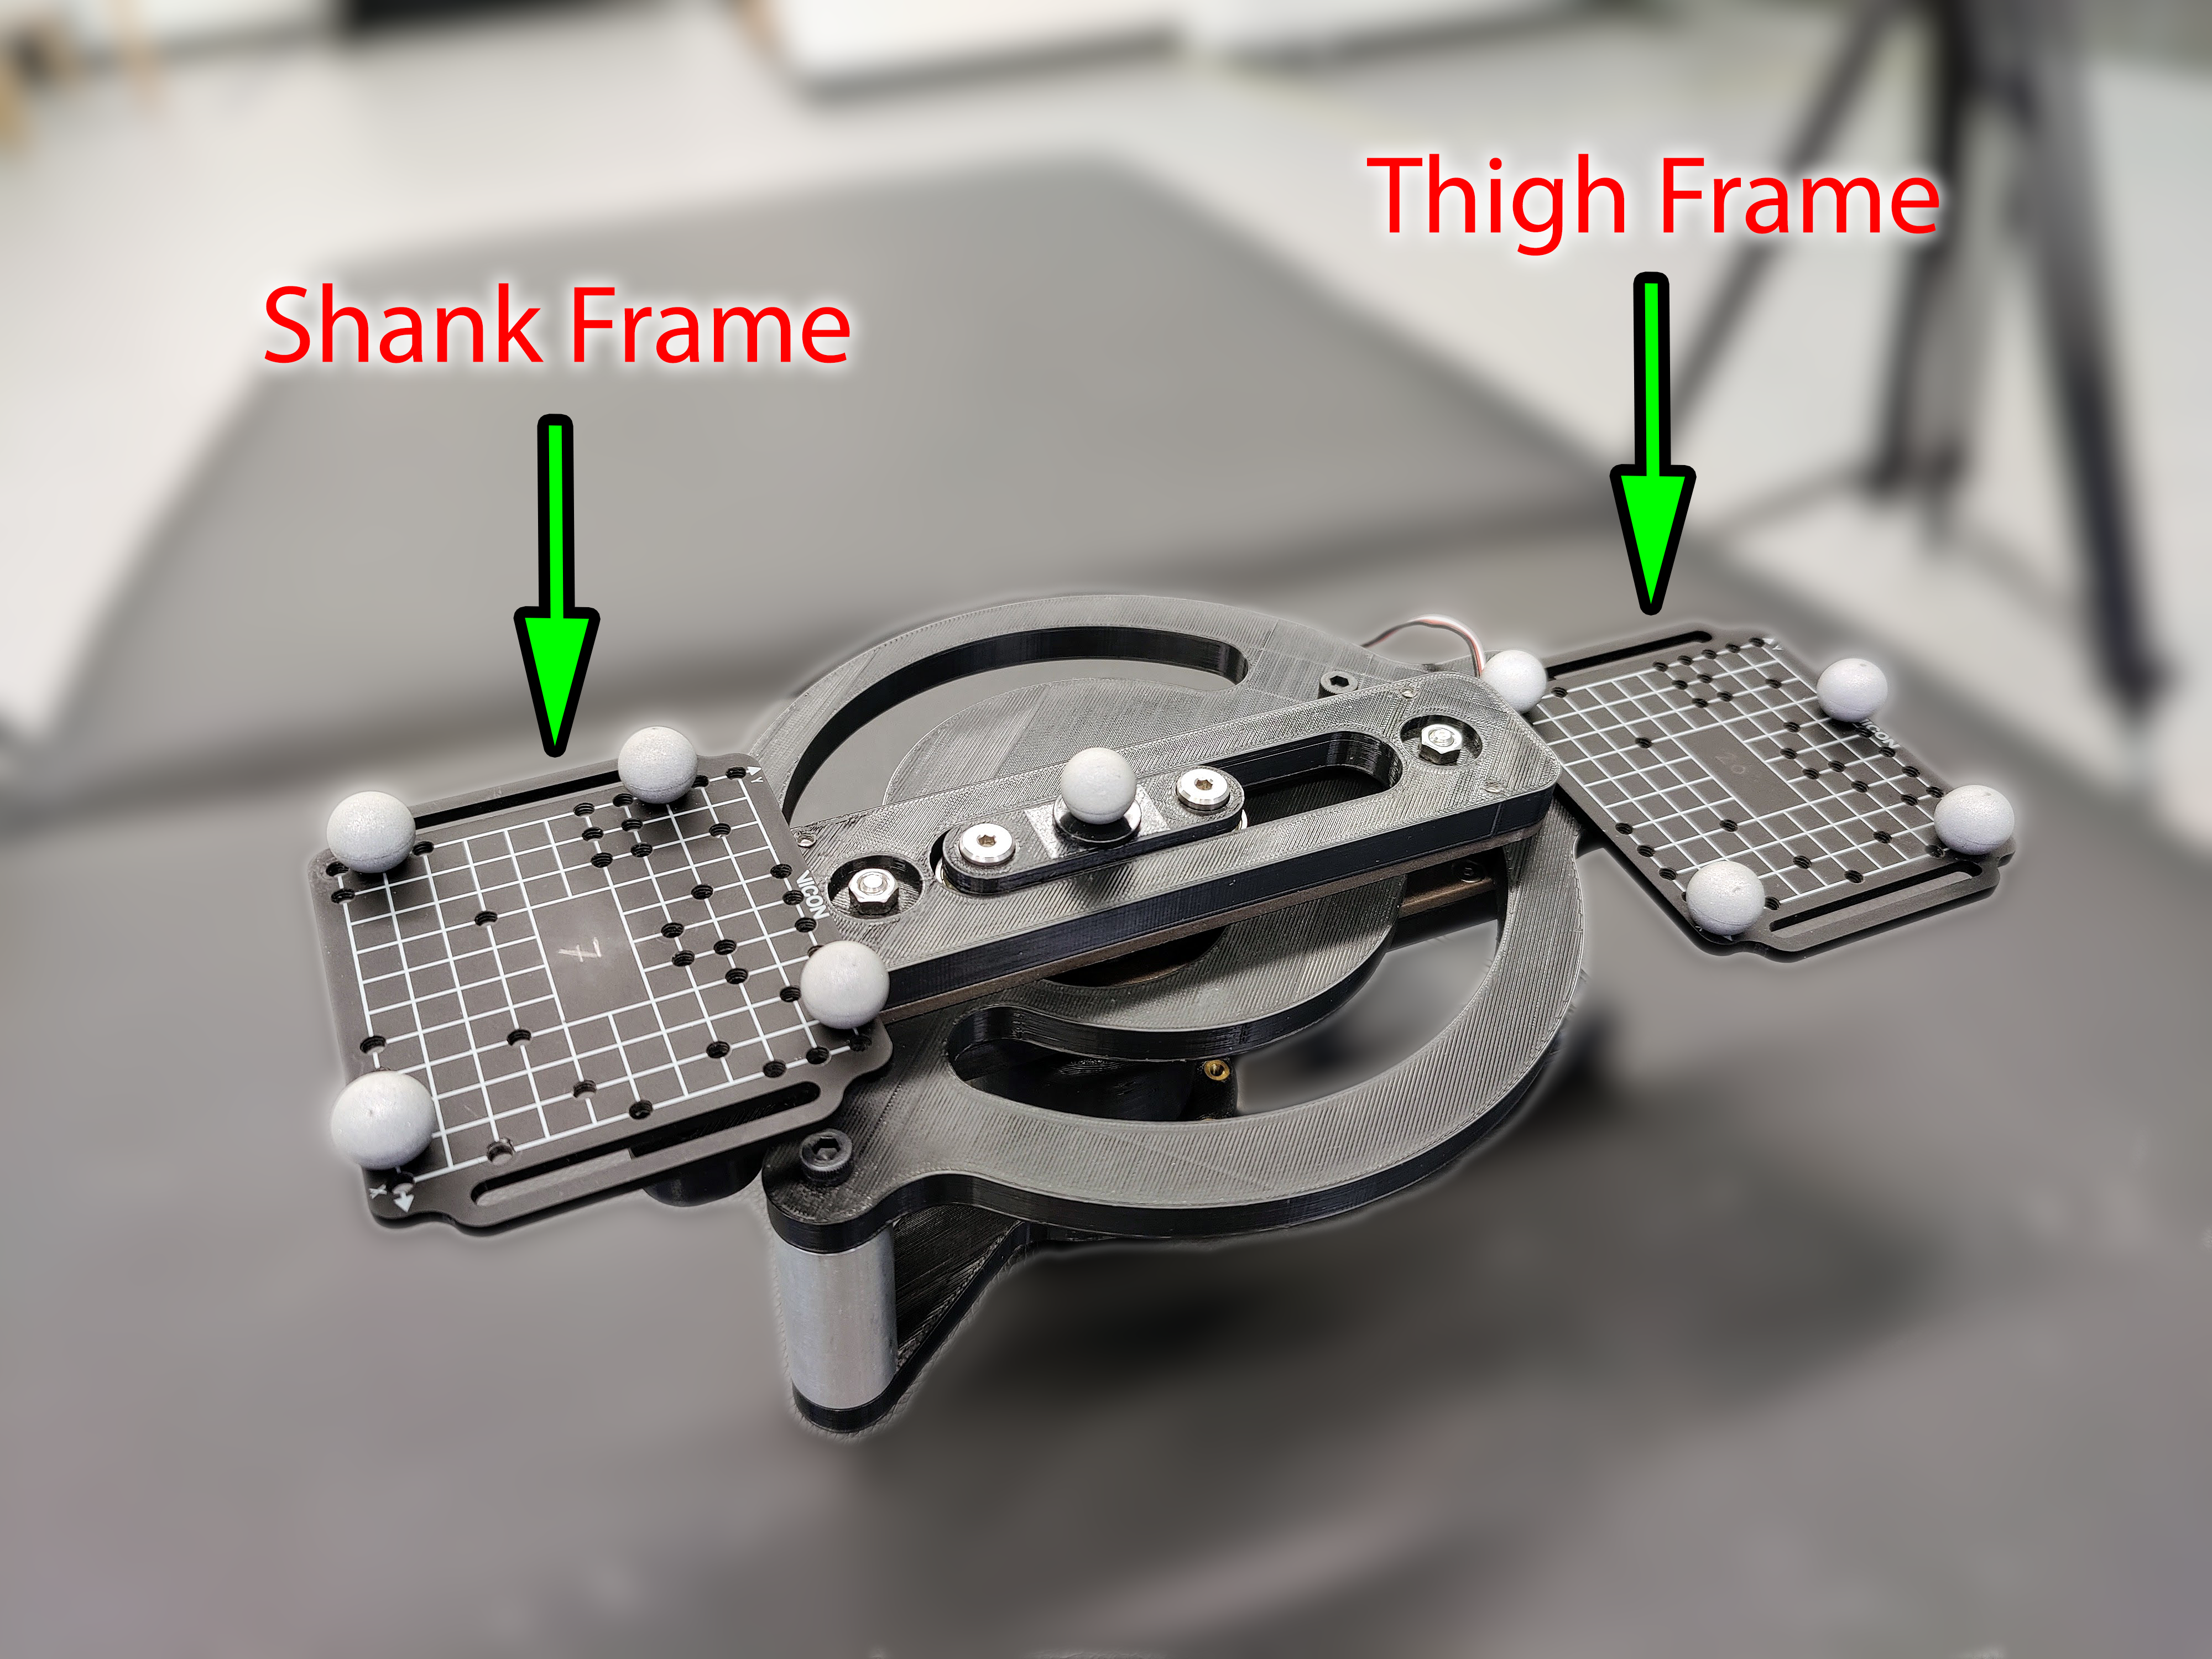
\includegraphics[width=0.8\linewidth]{Figures/Design/KneeTrajTest.png}
    \caption{Experimental setup for measuring the trajectory of the manufactured joint. 9 motion capture dots were used to measure any movement in all 6 degrees of freedom.}
    \label{fig:TrajTestSetup}
\end{figure}

To further verify the relationship, a 10-camera Vicon Vantage 5 motion capture system was used. 9 motion capture dots were placed strategically around the knee joint. Two rigid bodies were used (each containing 4 motion capture dots) to be able to measure position and orientation in all 6 degrees of freedom. One rigid body was placed on the connector on the shank link, while the other was attached to the connector of the thigh link. A final motion capture dot was placed at the joint center. Then, the joint was manually actuated through its range while collecting data from the motion capture system. The data was processed using software tools developed in \autoref{sec:KneeParams} for measuring human tibiofemoral relationships. To ensure the data collected remained representative of the test and was not modified by any processing tools developed, only data importing tools were used. These tools simply took the raw data from the Vicon system and imported it into Python in a cleaner way.

\begin{figure}[ht!]
    \centering
    \includegraphics[width=0.8\linewidth]{Figures/Design/FlexionExtensionKneeJoint.png}
    \caption{Results from the motion capture system demonstrates that the designed knee joint can follow a desired trajectory very closely, only deviating by \(1mm\) maximum}
    \label{fig:TrajTestResults}
\end{figure}

The motion capture analysis data in \autoref{fig:TrajTestResults} demonstrates the effectiveness of the joint; it was able to follow the desired trajectory layed out in \autoref{eq:KneeJointGeometryEquation} with minimal error (deviation from goal trajectory under \(1mm\)). 

    \chapter{Parameterization of Human Knee Joints}
\label{sec:KneeParams}

% Remember to talk about contributions to the Vicon packages (AIM_Vicon and AIM_GaitCore)

\TODO[inline]{Add knee parameterization once research is mostly concluded}

    \chapter{Conclusion \& Future Work}

\section{Conclusion}

\begin{figure}[ht!]
    \centering
    \includegraphics[width=0.7\linewidth]{Figures/KneeJointPrototype_ClearBackground.png}
    \caption{A picture of a left-sided knee joint prototype manufactured as a part of this thesis}
    \label{fig:KneeJointPicture}
\end{figure}

The proposed knee joint developed and tested in this thesis succeeded in all design requirements, even exceeding them in some scenarios. Experimentation showed that the knee could follow a defined tibiofemoral joint trajectory within \(1mm\) of accuracy. The joint itself can also be easily customized to each patient, with only one custom part needing to be manufactured per person per joint. Integrated sensors allow it to sense joint position and report it to the WPI LARRE hardware controllers. Strength analysis demonstrated that the joint can be manufactured from either PLA plastics using a conventional FDM 3D printer or machined out of aluminum. The joint will be able to support the stresses that come from common rehabilitation exercises including sit/stand exercises and walking gait exercises. Finally, the joint will be able to be integrated in the WPI LARRE (Legged Articulated Robotic Rehabilitation Exoskeleton). However, the design proposed is not limited to exoskeletons; the concept of using a cam mechanism to match tibiofemoral relationships can be applied to other orthoses that need to be powered.

\begin{figure}[ht!]
    \centering
    % \missingfigure[]{Picture of Knee Joint}
    \includegraphics[width=0.4\linewidth]{Figures/FinalExoRender.png}
    \caption{Proposed knee joint mounted to a model of WPI LARRE}
    \label{fig:KneeOnExo}
\end{figure}

% TODO: Add conclusion for the knee parameterization

\section{Future Work}

While the design was able to match and even exceed the design requirements, more research is needed. From a design perspective, the joint can be made much smaller than the existing design. The motor and gearbox can be integrated in the joint to offer a lower profile exterior. Additionally, a more efficient and less expensive no-backlash gearbox such as a cycloidal gearbox can be integrated to replace the {Harmonic\texttrademark} gearbox used in this study. 

Additionally, more research is needed in knee movement in an exoskeleton. The research discussed in \autoref{sec:KneeModel} demonstrates the relationship between the tibia and femur, and does not look how skin movement changes the trajectory. Studies using the parameterization method discussed in \autoref{sec:KneeParams} may demonstrate a more accurate relationship to be used with this knee joint, as well as determine the parameters of a patient's knee. This would create a future where a lower-limb paralysis patient would be able to receive a perfectly personalized knee joint for their rehabilitation exoskeleton using an imaging system. 
    
    % Print Bibliography
    \printbibliography[heading=bibintoc]

    \appendix

\chapter{Joint Power/Torque/Speed Calculations}
\label{apx:JointPowerTorqueSpeedCalcs}


\begin{table}[H]
    \centering
    \begin{tabular}{||c|c|c||}
        \hline
        Input (Motor) Power & \(P_{input}\) & \(90 Watts\) \\
        \hline
        Input (Motor) Torque @ Nominal & \(\tau_{input}\) & \(0.560 Nm\) \\
        \hline
        Input (Motor) Speed @ Nominal & \(\omega_{input}\) & \(2510 rpm\) \\
        \hline
        Input (Motor) Stall Torque & \(\tau_{in\_stall}\) & \(7.480 Nm\) \\
        \hline
        Gearbox Ration & \(\frac{n_1}{n_2}\) & \(100:1\) \\
        \hline
    \end{tabular}
    \caption{Motor/Gearbox Specifications}
    \label{table:ApxMotorGearboxSpecs}
\end{table}

\subsubsection{Power Calculation}
\begin{equation}
    P_{output} = \epsilon P_{input} = 0.9 * 90W = 81W
     \label{eq:PowerCalc}
\end{equation}

\subsubsection{Torque Calculation}
\begin{equation}
    \tau_{output} = \epsilon  \tau_{input} \frac{n_1}{n_2} = 0.9 * 0.560 Nm * \frac{100}{1} = 50.4 Nm
    \label{eq:TorqueCalc}
\end{equation}

\subsubsection{Speed Calculation}
\begin{equation}
    \omega_{output} = \omega_{input}  \frac{n_2}{n_1} = 2510 rpm * \frac{100}{1} = 2.510 rpm = 15^\circ/sec
    \label{eq:SpeedCalc}
\end{equation}

\begin{table}[H]
    \centering
    \begin{tabular}{||c|c|c||}
        \hline
        Output Power & \(P_{output}\) & \(81 Watts\) \\
        \hline
        Output Torque @ Nominal & \(\tau_{input}\) & \(50.4 Nm\) \\
        \hline
        Output Speed @ Nominal & \(\omega_{input}\) & \(15^\circ/sec\) \\
        \hline
        Output Stall Torque & \(\tau_{out\_stall}\) & \(673.2 Nm\) \\
        \hline
    \end{tabular}
    \caption{Joint Output Specifications}
    \label{table:ApxJointSpecs}
\end{table}

\chapter{Maxon Motor EC90 Datasheet}
\label{apx:EC90Datasheet}
Below is the datasheet for the motor chosen for this project: Maxon EC90 part number 429271 (highlighted)
\includepdf[]{Appendix/EC90_Specs.pdf}



\end{document}